\documentclass{acm_proc_article-sp}
\usepackage{tikz}
\usetikzlibrary{plotmarks}
\begin{document}
\title{Algorithm and Data Structure Coursework: \\PCA Features for
R-tree Based Similar Image Search}
\subtitle{}
%
\numberofauthors{2} %  in this sample file, there are a *total*
% of EIGHT authors. SIX appear on the 'first-page' (for formatting
% reasons) and the remaining two appear in the \additionalauthors section.
%
\author{\alignauthor
Qiwei Feng\\
       \affaddr{2011011250, IIIS-10}\\
       \affaddr{Tsinghua University}\\
       \email{gdfqw93@163.com}
\alignauthor
Pufan He\\
       \affaddr{2011011307, IIIS-10}\\
       \affaddr{Tsinghua University}\\
       \email{hpfdf@126.com}
}
\date{26 May 2015}

\maketitle
\begin{abstract}
This project implements a similar image search engine based on R-Tree and
several image features. We explores the performance of three major features,
i.e., color moment (by color distribution), principal component analysis (PCA,
by image rough shape), and K-Means (by image details). We analyzes the
correctness of different features, and the relation between features and R-Tree
node accessing times. We try different insertion orders and similarity
functions for R-Tree, and summarize their effect with different features.

We made our work open, and the full project codes can be found at \texttt{https://github.com/caiwaifung/lastcourse}.
\end{abstract}

\keywords{R-Tree, Similar Image, PCA, K-Means}

\section{Introduction}
Similar image searching is a popular problem in computer vision and data
science. Many nice approaches have been serving the public online, like Google,
Baidu, etc. The idea of fast and nice similar image searching usually splits
into two parts: feature extraction and close points finding.

\textbf{Feature extraction}: When calculating the similarity between two
images, we must find their simplified representation before we could compare,
because image dataset is too large. Usually the representation is an array of
integer or real numbers (feature vector). By representation, the similarity can
be simplified by some simple math operations between the representation
instead. The way to represent an image is called feature extraction. A well
designed feature should have two properties.
\begin{itemize}
\item Small. Smaller feature size means less stress on computation and storage.
\item Accurate. Similar images will have similar features, while irrelated
        images have discriminable features.
\end{itemize}

\textbf{Close points finding}: After all images have been turned into feature
vectors, the problem now is to maintain a set of vectors (image pool), and when
take a query vector (query image), find the top several closest vectors in the
set for the query one. This problem usually occurs in two scenario:
\begin{itemize}
        \item Sparse. E.g., many elements in a feature is zero, only some
                appears non-zero. Like the word count for a article. Usually an
                article will not cover all vocabularies we cares. We usually
                use inverse lookup based data structures to solve sparse
                feature similarity searching problem.
        \item Dense. The dimension of features are usually small, and most
                elements do not have default values that appears in a
                considerable probability. The features studied in this project
                are all dense features. We usually use K-D Tree based data
                structure to solve dense feature similarity searching problem.
                R-Tree is a variation of K-D Tree that is designed for disk
                structure.
\end{itemize}

\section{Feature Finding}
\subsection{Low Level Features}

We can design features for general images, with no training phase. Such
features are called low level features. However not to misunderstand, low level
features can be very strong.

\textbf{Color moment} is a low level feature: it considers each pixels color
space, RGB or HSV, and calculates the mean, variance, and skewness for each parts.
We included the given color moment feature in our project.
\begin{align}
        M^H_1&=\frac{1}{w\times h}\sum_{x,y}H[x,y]\\
        M^H_2&=\sqrt{\frac{1}{w\times h}\sum_{x,y}(H[x,y]-M_1)^2}\\
        M^H_3&=\sqrt[3]{\frac{1}{w\times h}\sum_{x,y}(H[x,y]-M_1)^3}
\end{align}
And similarly for $M^S_{1\dots 3}$ and $M^V_{1\dots 3}$. The final
representation is $\mathbb{R}^9$:\[\left\{M^H_{1\dots 3}, M^S_{1\dots 3},
M^V_{1\dots 3}\right\}\]
This feature describes the color distribution of image, without regard to the
pixel permutation.

There are many other way to design low level features like color space histogram,
gradient distribution or histogram, or we can divide the image into determined
districts, e.g. 3x3, and extract feature for each region, finally merge into a
single long feature.

However, low level features usually takes fixed size (dimension) and not
suitable for our study of R-Tree with different feature dimensions. So we tried
to extract deeper features that is learned from the dataset unsupervisedly (The
project guide forbids training feature with ground truth label).

\subsection{Principle Component Analysis}
A straight forward idea of comparing two image, is to resize them into an
identical size $w\times h$, and compare the images pixel by pixel. We set
$w=h=32$ which we think manually examining images is still feasible. All images
are resized to 32x32 in advance, with linear stretch if the ratio is not 1:1.

Because we already have color based feature, we leave out the color, and only use 32x32 $0~255$
grayscale images in this feature design.

Then, we can use a small set of 32x32 eigen images, as the principle
component learned from the dataset, to describe any potential image as close as
possible.

Every image can be written by a linear combination of several eigen images.
Eigen images are orthogonal with each other, so by dot production, we can
easily find the eigen base representation of a image.

PCA is to find eigen images in a way that first few eigen images will covers
the most variance of images in the data distribution.

We list the average image and first few principle components found by PCA in
our project:

\begin{tabular}{p{1.3cm}p{6cm}}
    Mean: &
\includegraphics[width=20pt]{../data/PCA_visualize/eigvec0.png} \\ 
    Eigen Images: &
        
\includegraphics[width=20pt]{../data/PCA_visualize/eigvec1.png}
        
\includegraphics[width=20pt]{../data/PCA_visualize/eigvec2.png}
        
\includegraphics[width=20pt]{../data/PCA_visualize/eigvec3.png}
        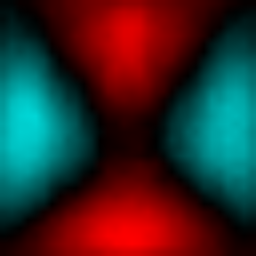
\includegraphics[width=20pt]{../data/PCA_visualize/eigvec4.png}
        
\includegraphics[width=20pt]{../data/PCA_visualize/eigvec5.png}
        
\includegraphics[width=20pt]{../data/PCA_visualize/eigvec6.png}
        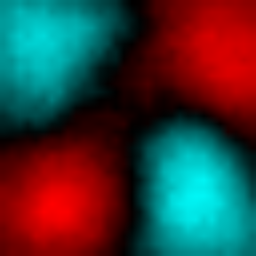
\includegraphics[width=20pt]{../data/PCA_visualize/eigvec7.png}
        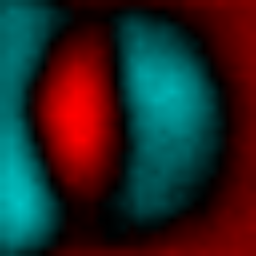
\includegraphics[width=20pt]{../data/PCA_visualize/eigvec8.png}
        
\includegraphics[width=20pt]{../data/PCA_visualize/eigvec9.png}
        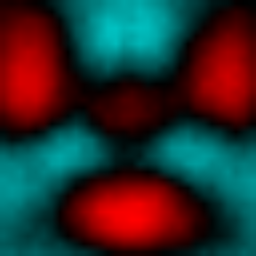
\includegraphics[width=20pt]{../data/PCA_visualize/eigvec10.png}
        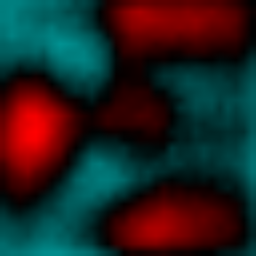
\includegraphics[width=20pt]{../data/PCA_visualize/eigvec11.png}
        
\includegraphics[width=20pt]{../data/PCA_visualize/eigvec12.png}
        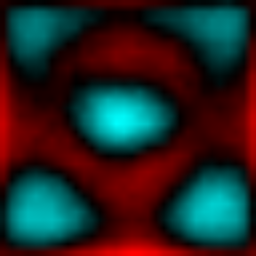
\includegraphics[width=20pt]{../data/PCA_visualize/eigvec13.png}
        
\includegraphics[width=20pt]{../data/PCA_visualize/eigvec14.png}
        
\includegraphics[width=20pt]{../data/PCA_visualize/eigvec15.png}
        
\includegraphics[width=20pt]{../data/PCA_visualize/eigvec16.png}
    \\
\end{tabular}

Note: Red means possitive, Cyan means negative. Dark means less absolute value.

The advantage of PCA is we can select to use any number of eigen images, i.e.,
only use the first few most significant components to represent the whole image
constitution. We used Numpy and Matlab in the training phase of PCA, which
takes just few minutes on a personal computer.

\subsection{K-Means}
Many research in computer vision finds that the appearance of same patterns
by convolution in image will help learning deep representation. K-Means is the
basic way to find such patterns.

First resize the images reserving the ratio to have the largest side length
$\leq 32$. Then we extract all 4x4 patches with RGB color space. So a patch
contains $48$ numbers, and for a resized image, there are at most
$(32-4+1)^2=841$ patches. We normalize each patch vector by
\begin{itemize}
\item Subtract the average among all 48 channels.
\item Normalize to a unit vector.
\end{itemize}
Then, we try to cluster all patches in the dataset (approximately $5613\times
841$) using $K$ centroids, for $K=4,8,12,16,20,24$.

Then we represent an image by $K$ average distances between every centroid and
all normalized patches that image has.

The training phase takes several hours, and that's why we only use $32$ image
side and $4\times 4$ kernel.

\subsection{Composite Feature}
We also designed a composite feature: the concatenation of PCA16 and
Color Moment. We adjust the scale of Color Moment by $0.1$ to balance the
feature variance.

\section{Data}

There are 5613 images given. We first random shuffle the dataset to $r_{0\dots
5612}$, and split
into two parts: pool set with 5000 size, query set with 613 size.
\begin{verbatim}data1k: 0~999; data2k: 0~1999; data3k: 0~2999;
data4k: 0~3999; data5k: 0~4999; query: 5000~5612\end{verbatim}

\section{R-Tree}
We use the ``rtree alternative package'' implementation of R-tree.
The wrapper \texttt{src/a.cpp} calls methods of provided R-tree class.
Run \texttt{python src/run.py} to compile and run the program.

\section{Experiments}

\subsection{Node Access Numbers}
\emph{Note: this is \textbf{problem 1}.}

Table~\ref{table:accessnum} lists the node access number in different cases.
\begin{table} \centering 
\begin{tabular}{|p{2.1cm}|c|c|c|c|c|}
    \hline
    Method and Feature Num & 1000 & 2000 & 3000 & 4000 & 5000 \\ \hline
    Color Moment HSV 9 & 46.11 & 67.69 & 88.69 & 98.24 & 117.0 \\ \hline
    PCA 4 & 37.18 & 53.31 & 71.37 & 76.72 & 81.83 \\ \hline
    PCA 8 & 68.42 & 107.7 & 145.8 & 176.1 & 208.4 \\ \hline
    PCA 12 & 77.95 & 129.9 & 174.5 & 217.8 & 252.6 \\ \hline
    PCA 16 & 82.46 & 135.4 & 190.2 & 236.2 & 280.0 \\ \hline
    PCA 20 & 81.55 & 137.8 & 196.4 & 253.7 & 302.8 \\ \hline
    PCA 24 & 83.11 & 135.7 & 192.8 & 248.0 & 297.4 \\ \hline
    PCA 30 & 123.8 & 207.4 & 281.4 & 351.7 & 416.4 \\ \hline
    KMeans 4 & \textbf{16.01} & \textbf{19.76} & \textbf{22.24} &
    \textbf{23.53} & \textbf{24.71} \\ \hline
    KMeans 8 & 17.49 & 21.83 & 24.44 & 25.88 & 26.66 \\ \hline
    KMeans 12 & 20.90 & 25.76 & 30.96 & 34.85 & 37.43 \\ \hline
    KMeans 16 & 22.22 & 28.40 & 33.89 & 37.25 & 38.14 \\ \hline
    KMeans 20 & 25.25 & 35.26 & 39.25 & 39.67 & 44.48 \\ \hline
    KMeans 24 & 20.68 & 27.81 & 30.20 & 33.46 & 34.79 \\ \hline
    Composite 25 & 80.01 & 136.8 & 202.4 & 254.9 & 305.4 \\ \hline
\end{tabular}
    \caption{Node Access Numbers}
    \label{table:accessnum}
\end{table}

Figure~\ref{fig:accessnum} shows the relationship between node access number
    and feature number
    under database of 5000 features.
\begin{figure} \centering
    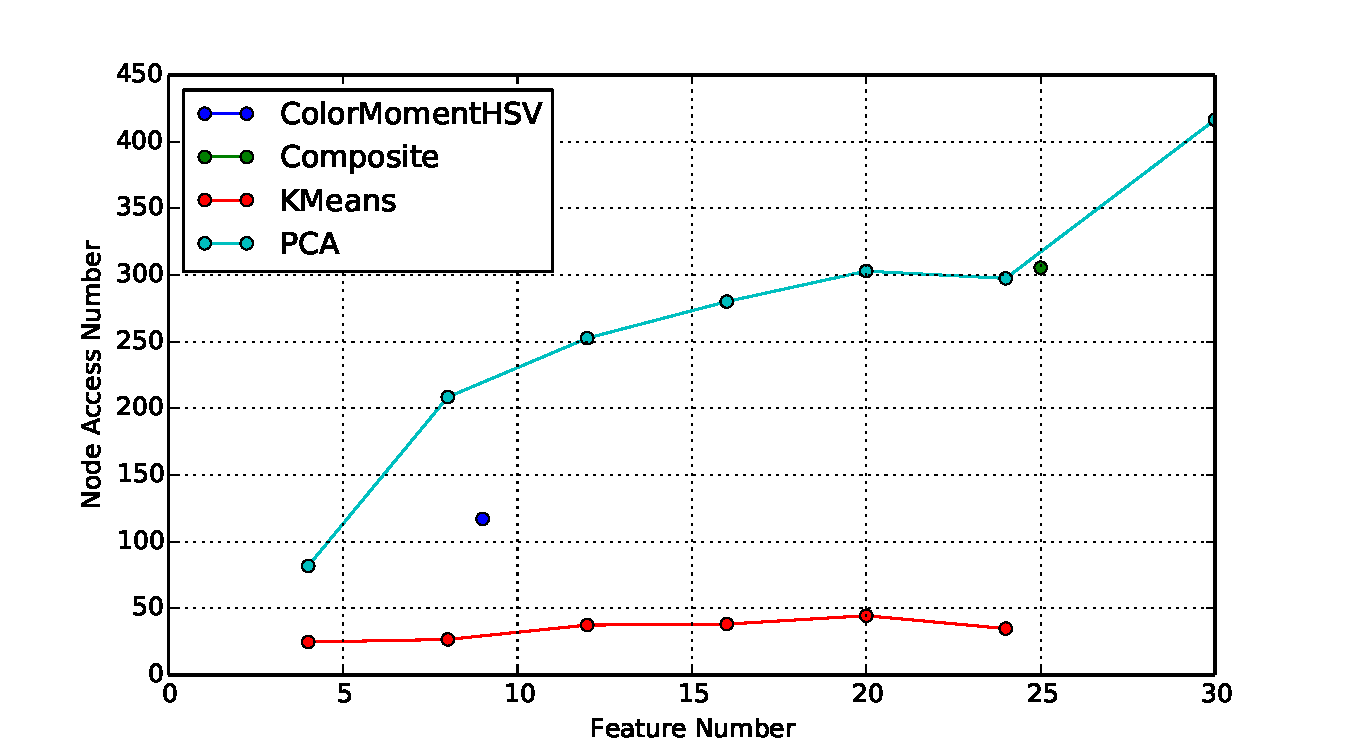
\includegraphics[width=0.4\textwidth]{data/accessnum.pdf}
    \caption{Node Access Number}
    \label{fig:accessnum}
\end{figure}
We can see that the number of access number increases while
    the feature number is increased.

\subsection{Performance}
\emph{Note: this is \textbf{problem 2}.}

Table~\ref{table:correctness} lists the correctness for different feature.
There are 613 queries in total, and the database varies from 1000 images
    to 5000 images.
The table shows that for each test case,
    how many nearest neighbors are in the same catalogy as
    the query image.
\begin{table} \centering 
\begin{tabular}{|p{2.1cm}|c|c|c|c|c|}
    \hline
    Method and Feature Num & 1000 & 2000 & 3000 & 4000 & 5000 \\ \hline
    Color Moment HSV 9 & 153 & 174 & 178 & 190 & 195 \\ \hline
    PCA 4 & 116 & 130 & 133 & 141 & 151 \\ \hline
    PCA 8 & 158 & 170 & 172 & 176 & 183 \\ \hline
    PCA 12 & 181 & 190 & 199 & 205 & 208 \\ \hline
    PCA 16 & 181 & 198 & 205 & 206 & 217 \\ \hline
    PCA 20 & 185 & 200 & 207 & 213 & 225 \\ \hline
    PCA 24 & 180 & 194 & 201 & 212 & 221 \\ \hline
    PCA 30 & 177 & 198 & 205 & 203 & 217 \\ \hline
    KMeans 4 & 126 & 132 & 147 & 148 & 147 \\ \hline
    KMeans 8 & 124 & 155 & 154 & 155 & 161 \\ \hline
    KMeans 12 & 132 & 154 & 158 & 154 & 158 \\ \hline
    KMeans 16 & 133 & 154 & 165 & 167 & 173 \\ \hline
    KMeans 20 & 132 & 160 & 157 & 159 & 164 \\ \hline
    KMeans 24 & 121 & 161 & 153 & 167 & 178 \\ \hline
    Composite 25 & \textbf{201} & \textbf{219} & \textbf{230} & \textbf{235} &
    \textbf{240} \\ \hline
\end{tabular} 
\caption{Correctness of Different Feature}
\label{table:correctness}
\end{table}

\subsection{The Results}
\emph{Note: this is \textbf{problem 3}. }

Figure~\ref{fig:result} shows some sample results from both
    Color Moment HSV 9 features and
    Composite 25 features.
Here are three sample queries.
The first, third, and fifth rows in the figure
    is the results from Composite 25 features,
    while the second, the forth, and the sixth
    rows is from Color Moment HSV 9 features.
In each row, the first picture is the query,
    and the following are five best answers according to
    their relevance to the query.
A tick indicates that the answer to its left is correct,
    i.e., in the same catalogy of the query.
\begin{figure} \centering
    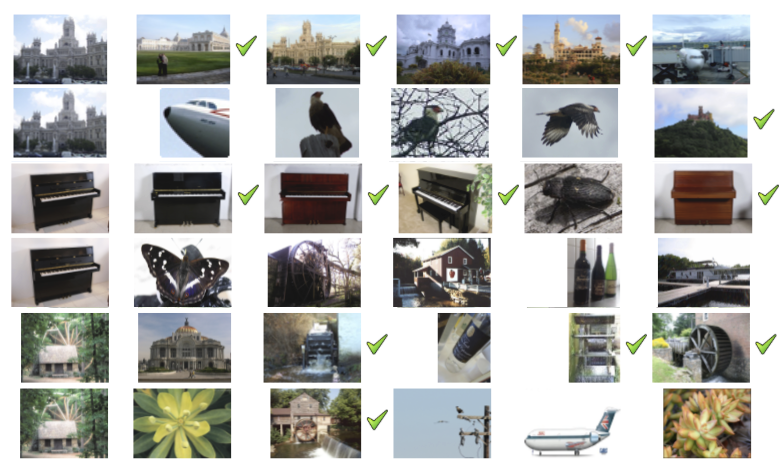
\includegraphics[width=0.45\textwidth]{data/result.png}
    \caption{Sample Nearest Neighbors}
    \label{fig:result}
\end{figure}

In the first example, the query is a big house.
The Composite method finds 4 buildings in the top-5 nearest neighbor searching.
The Color Moment HSV method, however, finds many
    irrelevant pictures.
In the second example, the Composite method
    also finds 4 piano which is the correct.
The HSV method fails to find any piano in its
    5 nearest neighbor searching process.
The thrid example is a waterweel.
Both the Composite method and the HSV methods make mistakes
    in this example,
    but the Composite method still does better
    by making three ticks in five answers.

Please see \texttt{demo.html} under \texttt{result.zip} for a more detailed demo.

\subsection{Other Similarity Functions}
We tried two other similarity functions and their comparison
    with standard Euclidean distance similarity function is shown
    in table~\ref{table:simfunc}.
\begin{table} \centering 
\begin{tabular}{|c|c|c|c|c|}
    \hline
    Function & HSV9 & PCA8 & PCA16 & Composite \\ \hline
    $\sqrt{\sum_i (a_i - b_i)^2}$ & 171 & 177 & 205 & 229 \\ \hline
    $\sum_i |a_i - b_i|$ & 179 & 176 & 201 & 237 \\ \hline
    $\frac{\sum_i a_i b_i}{||a|| ||b||}$
    & 167 & 160 & 197 & 232 \\ \hline
\end{tabular} 
\caption{Difference Similarity Functions}
\label{table:correctness}
\end{table}
We can see that under certain feature methods,
    the absolute difference similarity function (second one) performs better
    than the Euclidean distance similarity (first one) function.
Meanwhile, the cosine similarity (third one) function
    is worse than two other functions.

\nocite{*}
\bibliographystyle{abbrv}
\bibliography{sigproc} 

\balancecolumns

\end{document}
